%% 该模板修改自《计算机学报》latex 模板
%% 主要是将双栏改成单栏，去掉了部分计算机学报标识；
%% 源文件自：https://www.overleaf.com/latex/templates/latextemplet-cjc-xelatex/ybmmymncrrmw
%%
%%
%% This is file `CjC_template_tex.tex',
%% is modified by Zhi Wang (zhiwang@ieee.org) based on the template
%% provided by Chinese Journal of Computers (http://cjc.ict.ac.cn/).
%%
%% This version is capable with Overleaf (XeLaTeX).
%%
%% Update date: 2023/03/10
%% -------------------------------------------------------------------
%% Copyright (C) 2016--2023
%% -------------------------------------------------------------------
%% This file may be distributed and/or modified under the
%% conditions of the LaTeX Project Public License，either version 1.3c
%% of this license or (at your option) any later version.
%% The latest version of this license is in
%%    https://www.latex-project.org/lppl.txt
%% and version 1.3c or later is part of all distributions of LaTeX
%% version 2008 or later.
%% -------------------------------------------------------------------

\documentclass[10.5pt,compsoc,UTF8]{CjC}
\usepackage{CTEX}
\usepackage{graphics}
\usepackage{graphicx}
\usepackage{footmisc}
\usepackage{subfigure}
\usepackage{url}
\usepackage{multirow}
\usepackage{multicol}
\usepackage[noadjust]{cite}
\usepackage{amsmath,amsthm}
\usepackage{amssymb,amsfonts}
\usepackage{booktabs}
\usepackage{color}
\usepackage{ccaption}
\usepackage{booktabs}
\usepackage{float}
\usepackage{fancyhdr}
\usepackage{caption}
\usepackage{xcolor,stfloats}
\usepackage{comment}
\setcounter{page}{1}
\graphicspath{{figures/}}
\usepackage{cuted}%flushend,
\usepackage{captionhack}
\usepackage{epstopdf}
\usepackage{gbt7714}
\usepackage{adjustbox}

%===============================%

% \headevenname{\mbox{\quad} \hfill  \mbox{\zihao{-5}{ \hfill 《课程名称》  } \hspace {50mm} \mbox{■■■■ 年 ■■ 月}}}%
\headevenname{\mbox{\quad} \hfill  \mbox{\zihao{-5}{ \hfill Touhou Stellar Chronicles ~ Symphony of Phantasm  }}}%
\headoddname{\hfill Touhou Stellar Chronicles ~ Symphony of Phantasm}%

%footnote use of *
\renewcommand{\thefootnote}{\fnsymbol{footnote}}
\setcounter{footnote}{0}
\renewcommand\footnotelayout{\zihao{5-}}

\newtheoremstyle{mystyle}{0pt}{0pt}{\normalfont}{1em}{\bf}{}{1em}{}
\theoremstyle{mystyle}
\renewcommand\figurename{figure~}
\renewcommand{\thesubfigure}{(\alph{subfigure})}
\newcommand{\upcite}[1]{\textsuperscript{\cite{#1}}}
\renewcommand{\labelenumi}{(\arabic{enumi})}
\newcommand{\tabincell}[2]{\begin{tabular}{@{}#1@{}}#2\end{tabular}}
\newcommand{\abc}{\color{white}\vrule width 2pt}
\renewcommand{\bibsection}{}
\makeatletter
\renewcommand{\@biblabel}[1]{[#1]\hfill}
\makeatother
\setlength\parindent{2em}
%\renewcommand{\hth}{\begin{CJK*}{UTF8}{gbsn}}
%\renewcommand{\htss}{\begin{CJK*}{UTF8}{gbsn}}


\begin{document}

\hyphenpenalty=50000
\makeatletter
\newcommand\mysmall{\@setfontsize\mysmall{7}{9.5}}
\newenvironment{tablehere}
  {\def\@captype{table}}

\let\temp\footnote
\renewcommand \footnote[1]{\temp{\zihao{-5}#1}}


\thispagestyle{plain}%
\thispagestyle{empty}%
\pagestyle{CjCheadings}

% \begin{table*}[!t]
\vspace {-13mm}


\onecolumn
\zihao{5-}\noindent Touhou Stellar Chronicles ~ Symphony of Phantasm\\
\noindent\rule[0.25\baselineskip]{\textwidth}{1pt}

% \onecolumn
% \zihao{5-}\noindent 第??卷\quad 第?期 \hfill 计\quad 算\quad 机\quad 学\quad 报\hfill Vol. ??  No. ?\\
% \zihao{5-}
% 20??年?月 \hfill CHINESE JOURNAL OF COMPUTERS \hfill ???. 20??\\
% \noindent\rule[0.25\baselineskip]{\textwidth}{1pt}

{
\centering
\vspace {11mm}
{\zihao{2} \heiti 东方繁星录~Symphony of Phantasm设定v1.1 }

\vskip 5mm

%{\zihao{4}\fangsong 作者名$^{1)}$\quad  作者名$^{2),3)}$ \quad 作者名$^{3) }$($^*$字体为3号仿宋*作者)}

% \footnote{\noindent \zihao{6}
% % 收稿日期：\quad \quad -\quad -\quad ；最终修改稿收到日期：\quad \quad -\quad -\quad .*投稿时不填写此项*. 本课题得到… …基金中文完整名称(No.项目号)、… …基金中文完整名称(No.项目号)、… … 基金中文完整名称(No.项目号)资助.
% \textsf{作者名1}，学号，学位(或目前学历),主要研究领域为*****、****. E-mail: **************.\textsf{作者名2}，学号，学位(或目前学历),主要研究领域为*****、****. E-mail: **************. \textsf{作者名3}，学号，学位(或目前学历),主要研究领域为*****、****. E-mail: **************.}

\vspace {5mm}

\zihao{5}{这曾是一个没有人类记下历史的封闭世界。妖怪们无法准确记住过去，幻想乡里见不到真实。}

\zihao{5}{就在我开始写这本书的时候，幻想乡的历史就已经诞生了。}

\zihao{5}{那么，请仔细阅读吧，愿您有一个安全美好的幻想乡生活。}

\zihao{5}{by 第$\blacksquare$代$\blacksquare$$\blacksquare$$\blacksquare$$\blacksquare$}

% \zihao{6}{\textsf{论文定稿后，作者署名、单位无特殊情况不能变更。若变更，须提交签章申请，国家为中国可以不写，省会城市不写省名，其他国家必须写国家名。}}
}

\vskip 5mm

\zihao{5}{
\setlength{\baselineskip}{16pt}\selectfont{
\noindent {\heiti 概\quad 述\quad }
\textbf{东方繁星录 Mod} 基于 Stellaris 世界观，沿用游戏原版的\textbf{基础设定}并尽量不与其发生冲突。如果本设定中对原版设定做出了额外解释，则 \textbf{Mod 设定覆盖原版设定}，在没有额外解释的情况下，采纳设定的优先度为: \textbf{原版游戏设定 > 原版游戏表现}。本设定可以兼容其他 Mod 中不冲突的设定，但\textbf{不考虑与其他 Mod 的设定冲突}的情况，同时\textbf{不建议跨世界观论战}。对于未给出的设定,一切均以\textbf{东方一设或作为其创作原型的设定\textbf}为基准。本 Mod 的设定目前可能尚不完善，因此难免出现奇奇怪怪的 bug，如果你提出了合理的建议，将可以考虑采纳吸收。
\par}}
\vspace {5mm}

%\zihao{5}{\noindent
%{\heiti 关键词 \quad }{*关键词（中文关键字与英文关键字对应且一致，应有5-7个关键词)；关键词；关键词*  }
%}
% \zihao{5-}{\heiti 中图法分类号\quad } TP\rm{\quad \quad \quad     }
% {\heiti DOI号:\quad } *投稿时不提供DOI号


\vskip 7mm

\section{\heiti 宇宙相关}

\subsection{通用设定}

\zihao{5}{
\setlength{\baselineskip}{18pt}\selectfont{
{\bf 本 Mod 中的宇宙遵循以下设定:}
\zihao{5}{ 
	\begin{itemize}
		\item \textbf{真空光速}：真空光速仍然是有限的，各个文明也依旧不能够在以常规的方式来进行超光速航行。
		\item \textbf{宇宙起源及演化}：宇宙如同现实中的宇宙一样，起源于 137 亿地球年前的大爆炸，其膨胀、演化与各个时期
		的物质分布均与现实中的宇宙保持一致。
		\item \textbf{无神世界}： Mod 的世界观不承认任何形式的神存在，神仅仅作为具备可解释强大能力的个体存在而无神性，对于东方原作中的神采取“是灵力较为强大的
		个体，但仍需要信仰来维持自己存在”的设定。
	\end{itemize}
\par}}

\subsection{其他维度}

本章节中提及的其他维度均指\textbf{除了现实空间以外的维度}，其中由于博丽大结界和月面结界的特殊性质，幻想乡和里之月都不属于现实空间的一部分。

\subsubsection{\textcolor{purple}{魔界}}

本Mod设定中认定魔界为其他维度的空间，文案中的“\textbf{次元}”、“\textbf{位面}”等称呼均指代这一概念，并且魔界空间为魔界文明的神绮利用自身力量、科技与阴阳玉所开辟，可以通过星界裂隙等能穿越星界壁垒的方式来前往。一般认为现实空间中的坐标与魔界空间的坐标\textbf{一一对应}，二者时间流速一致，同时魔界位面的绝大多数物理定律均与现实空间一致。

初始的魔界空间仅为一片虚无，类似于现实空间中河系之间的虚空，但不存在任何星际介质。直到神绮借助自身的能力与科技设备近乎完美的复刻了整个超星系团，但是在本超星系团以外的空间依旧是一片虚无。

\subsubsection{结界空间}

与魔界类似，\textbf{所有的结界共同构成了结界空间}，但是从结界内部前往不同结界之间的虚无非常困难，这是结界建立的原理所导致的。此前博丽灵梦等人能够直接从博丽大结界内部前往月球上的月都结界内部，就是跨越了这一虚空，从而抵达另一片结界内部。结界空间的坐标与现实空间的坐标存在着某种复杂的关联关系，大致可以认为是\textbf{1：6.666}，并且基于此特性，月之都曾经开发出了借助结界空间进行航行的跃迁引擎，在目的地开辟一个短暂存在的结界，并且通过结界空间前往对应的现实空间坐标即可。

此外，在开辟结界之后，一套与现实空间中一模一样的\textbf{“子空间”}会在结界空间中出现，但是内部的改动\textbf{不会}在结界之外有任何反馈，除非混淆了\textbf{“真实与虚幻的结界”}。由于开辟与维持结界需要的灵力随着“子空间”体积的增大会\textbf{成倍的增长}，因此往往结界内部的空间不会太大，一般不超过整个星球的范围。同时由于结界的特殊性质，只有灵力能够稳定的开辟与维持其存在，其他的能量输入形式都或多或少的存在一些问题，也只有具备灵力的物种才能自如的驾驭这种力量了。

\subsubsection{\textcolor{red}{隙间}}

一片神秘的维度，无法通过隙间裂口以外的任何形式进入，而开辟隙间裂口又需要隙间妖怪所独有的能力，某种意义上这里是独属于隙间妖怪这一物种的空间。隙间维度的坐标与现实空间不存在任何对应关系，其使用者能够在现实空间的任意位置开辟隙间裂口，从而实现快速移动。其内部有一个无限拓展的漆黑平面，如液体的同时又如同固态物质，在这一平面上空的天空存在着一些诡异的紫色眼眸，时不时移动着，虽然漆黑但是始终投射着柔和而令人安心的光照。整片“星空”似乎近在咫尺又似乎远在天边，不论是靠近还是远离，其似乎都与观察者保持着一致的距离，神秘而又诡异。整个空间的大小目前没有任何已知边界，似乎可以无限向外拓展。

隙间中存在着一些很久之前的人造物体，似乎这片空间\textbf{不仅仅由八云紫使用过}。考虑到隙间能且仅能通过隙间裂隙进入，其他方式进入将会被强行排斥离开，着证明她也不是唯一的一位隙间妖怪，\textbf{至少曾经不是}。

\subsubsection{\textcolor{cyan}{二又二分之一次元}}

原型为《东方年代记》中出现的二又二分之一次元，本 Mod 基本设定与其一致,但被关押于其中的事物很难从中出去，对于其中的任意坐标,现实空间的对应坐标都为\textbf{同一点}，同时二者时间流速一致。

\subsubsection{\textcolor{violet}{虚境}}

现实空间中的每一个位置都与虚境，具体来说，是表层虚境中的一个位置\textbf{一一对应}，而在表层虚境以“下”，是\textbf{浅层虚境}和更“深”处的\textbf{深层虚境}。一般而言,越往虚境的“深”层,危险性越高。而大多数能够“进入虚境”的文明，接触到的便是\textbf{表层或者浅层虚境}。对于大多数文明来说，浅层虚境便已经足够危险,这里还存在着一些灵能极强的个体，甚至有可能会形成文明。其中一些灵能能力足够强大甚至能够在虚境中开辟属于自己的灵能领域，形形色色的大小超主就是这种强大存在的典型案例。在浅层虚境中存在着数个格外强大的存在，由于其灵能足以部分的干涉和影响现实空间，被一些文明称之为“超主”乃至“上超主”。而深层虚境，几乎没有太多文明能够进入其中还能安全离开。

事实上，深层虚境远比表层和浅层虚境要广袤的多，甚至可以让表层和浅层虚境都被忽略不计。深层虚境的灵能活动波涛汹涌，即使是短暂地进入这里，都有可能不幸因为突如其来的灵能环境变化而被立刻摧毁。深层虚境可以依照其活跃层度继续无限地分层，进入虚境越深，灵能活动越活跃，移动的连续性要求也越弱，当然，理论上没有任何东西能够进入虚境的最深处，那里近乎无穷大的能量会撕碎一切。有传闻说曾经有人观测到了\textbf{在深层虚境中活动的令人疯狂的生命体}，但是这种事情也仅仅被当成当事人受到灵能影响而影响了认知功能。

历史上，只有灵能能力极强的\textbf{泽洛文明}、以及\textbf{月之都当中的升格派}可以进入这里。然而泽洛文明升格派在与另一个文明的冲突之中，被福音派和他们拉出了虚境粉碎；月之都的升格派则不知所踪，\textbf{\textcolor{purple}{也许}}是消散在了深层虚境混乱的灵能活动当中，但是谁知道呢？。

此外，那些使用以太相引擎等手段试图让自己飞升的文明，失败者会被深层虚境所吞噬，而成功者也只能对表层虚境造成损伤,，至他们遗留下来的黑洞反而会滋养着深层虚境。

\subsection{\textcolor{magenta}{灵力}}

灵力是幻想相关的存在具备的一种能量形式，其可以被通过特殊手段存储与利用，灵力赋予了妖怪与部分人类那些看似不合常理的力量，而在使用这些力量时可以检测到一些独特的辐射特征。使用与存储灵力会对现实空间产生一些微弱而奇妙的影响，不过随着时间的流逝会自然的消散。有机体的一些特殊结构能够控制灵力，这也是妖怪与神明获得强大力量的根源，因此使用人造的类似结构去控制灵力是可行的，但是这要比常规的有机生物要困难的多，也需要耗费更多的能量。

\subsection{\textcolor{magenta}{幻想乡}}

幻想乡原先为现实世界的一部分，这个地理概念的存在至少超过了一千两百年。一开始幻想乡仅仅指的是远离人类村落的深山里的一片地方。直到某一天，由于人口的增加，为了恢复被人类压迫的妖怪在幻想乡的势力，能操纵界线的妖怪八云紫策划并实行了一次\textbf{妖怪扩张计划}，在原本的幻想乡周围创造了幻与实的界线，从逻辑上创造了今天意义上的幻想乡。

幻想乡与外面世界被包围幻想乡的结界分割，其中结界内是幻想的、非常识的部分，而结界外是现实的、常识的部分。由于被笼罩于博丽大结界内部的空间，其属于结界空间的一部分，数千年前贤者们通过自身的灵力将现实空间的一部分剥离进入了博丽大结界，但是现实空间对应的位置并没有发生实际上的改变。博丽大结界由现实与幻想、常识与非常识两条界线组成，其基本功能不仅有使被外面世界否定（消失、遗忘）的存在与力量流入幻想乡，还能阻止有意识的存在主动出入幻想乡。

作为与大结界内幻想乡直接相通的维度之一，地狱事实上也存在于结界空间，但是其通过特殊的结界隧道与幻想乡直接相连，在广义上也可以认为是幻想乡的一部分。三途河作为同时存在于彼岸与幻想乡的河流，分割着幻想乡与彼岸；而彼岸又能够通往地狱。同时，最特殊的是地狱同时与多个维度联通，但是不同维度的人们只能前往对应自己维度的那一部分地狱空间。因而地狱可以说是无限广阔，并且不同的地区环境差异极大。如无间地狱，其环境为空旷而一望无际的黑暗，地面无比荒芜，聚集了大量的骷髅。赫卡提亚曾提及了不同的地狱景象，包括血池地狱、针地狱、灼热地狱等等，但无论是哪个地狱都是一幅守旧不变寂寥荒芜的景象。

除了幻想乡、彼岸和地狱，还有冥界、异界和天界等许多与幻想乡联通或存在关联的维度，这些地方都属于结界之内，并且存在着妖怪、神明等曾经被否认的幻想生物，可以算作\textbf{幻想侧}的一部分。需要注意的是，虽然幻想乡内存在着现已无法使用的魔界大门，但魔界在实际上仍然算独立维度，而不是作为结界空间一部分存在。

\subsection{\textcolor{blue}{星界}}

严格来说星界并不算作某种单独存在的维度，而是无数次元和次元之间的势能壁垒构成的整体，这种势能壁垒一般被称呼为\textbf{\textcolor{blue}{星界壁垒}}。总体而言，玩家所处的时间节点上，星界壁垒的强度非常薄弱，有些情况下甚至能够自发的在两个次元的空间之间形成某种高维能量通道，即星界裂隙，这使得这一时期的文明跨越星界壁垒建立跨次元文明成为可能。但突破星界壁垒所需的能量仍然超出了绝大多数文明的技术水平，因此仅有某些如破界者这样的文明成功建立了跨次元帝国，并且之后分裂消亡了。

总的来说，星界壁垒的强度并不总是固定不变的，而是存在某种周期性的变化，只不过玩家所处的数千万年的短暂间隔期内，星界壁垒整体较为薄弱。过往曾经有数个先驱文明试图突破星界壁垒，前往其他次元定居，然而他们基本都失败了。某个未知文明在大麦哲伦星云发现的古代巨型结构$\blacksquare$$\blacksquare$曾经被另一个已经消失的先驱文明用于跨越任意两个次元之间的星界壁垒，然而由于此时的星界壁垒的能垒已经比之前高了一些，$\blacksquare$$\blacksquare$$\blacksquare$$\blacksquare$最终失败了，还造成了席卷整个$\blacksquare$$\blacksquare$$\blacksquare$$\blacksquare$星云的空间扭曲现象，直到现在该河系依旧是不宜居的。

\section{异变}

\textbf{破界者}\quad 高维恶魔，或称破界者，他们曾经建立过一个跨次元帝国，他们的社会在多个维度之间延伸，殖民整个宇宙，就像其他文明殖民新行星一样。然而，一切幻梦均有代价，他们脆弱的跨次元帝国基于某种星界管路结构，并且最终在超负荷运转后彻底湮灭，顺带着埋葬了整个帝国。实际上他们的这一技术并非由自己创造，而是在观测$\blacksquare$$\blacksquare$次元时，无意间发现了一组研究资料，正是关于用于刺破星界壁垒的古代巨型结构的。虽然仿制出来的质量远不如其原型，但能够勉强维持他们的那个小小帝国，直到负载过大而彻底崩溃。

\textbf{肃正协议}\quad 一个试图阻止所谓30级奇点威胁的星系内机械智能，它们自称是在星系刚刚诞生之时就已经存在，然而这实际上仅仅是其存储介质混乱导致的异常认知。实际上肃正协议的诞生远晚于那个时期，制造它们的河系内文明仅仅发现了一些超出想象的造物，以及一些可怕的景象，就误认为30级奇点会威胁宇宙。30级奇点可能存在危险，但一个连河系都没能出去的文明，本身甚至未能攻克五级奇点，去怀疑甚至担心这一点未免有些杞人忧天了。

\textbf{异变的传说}\quad 在曾经的幻想乡中，吸血鬼放出红雾也好、冬天和夜晚不会结束也好、都市传说真的发生也好、四季景象同时出现也好……这些幻想乡中不时发生的异常事件被称为\textbf{异变}。进入星际时代的幻想乡，理所当然的也遇到了各种各样新奇的异变……从道具的解放者、被释放游弋于虚空中的灵力实体，到野心勃勃的地狱中的妖怪们……\newline\newline\newline\newline\newline

\begin{center}
\zihao{3}{ \heiti 先驱文明}\\
\vspace {5mm}
\zihao{5-}{\color{gray}在宇宙诞生之后，曾经涌现过一批具备灵力的物种组建的先进文明}

\zihao{5-}{\color{gray}然而他们最终失去了踪迹}

\zihao{5-}{\color{gray}仅留下了一座座遗迹，宣示着她们的存在}

\zihao{5-}{\color{gray}其中埋藏的东西，或许能带来技术上的指引，也可能是席卷整个星系的灾难}

\end{center}

\section{隙间之里}

\subsection{\color{gray}概述}

实际上隙间妖怪并非一直都只有八云紫一人，隙间之里便是一个主要由隙间妖怪组成的远古文明，其人数稀少而高度依赖于自动化设施与智能机械。据信其成功使得人工智能也具备了灵力能力，并且使得合成人们能够代劳她们的大部分工作。与其他两个同时期文明不同，隙间之里似乎没有明确的势力范围，其影响力也较弱，但是其实际势力不容小觑。最终这个文明神秘的退出了银河系的舞台，没人知道她们是否仍然存在于某些地方，至少银河系中已经很长时间没有他们的活动迹象了。

\subsection{\color{gray}历史事件}

隙间之里的大致历史沿革如下：
\begin{itemize}
	\item \textbf{永恒的终结}：在星系的早期，隙间妖怪们借助自己的力量，模糊过去与未来的界限，发展了基于时间力场的时间技术，并且成立了永恒时空组织。这一组织旨在调整时间线，确保整个文明不会受到各种灾难的影响。然而好景不长，最终她们认识到了改写时间线的技术最终会使得文明发展停滞不前，选择在过去的某个时间点主动解散了永恒时空，并在时间线上防止时空障碍来阻止其他文明重蹈覆辙。虽然她们失去了永恒，但是也获得了踏入群星的机会。
	\item \textbf{开辟隙间}：
	\item \textbf{繁星门扉}：
	\item \textbf{浪迹虚空}：
	\item \textbf{机械黎明}：随着合成人技术的发展和文明规模的扩大，隙间之里军用舰队的人手不足的问题变得愈发严重起来。为此，她们对合成人阳电子脑的结构进行了修改，并且运用自己的灵力，赋予这些智能以使用灵力的能力。最终她们将大部分舰队都改组为了搭载军用人工智能单元的自动化舰队，而这无疑也为后面的一系列灾难埋下了伏笔。
	\item \textbf{智械叛乱}：
	\item \textbf{退出舞台}：
\end{itemize}

\subsection{\color{gray}典型技术}

\subsection{\color{gray}现状}

\section{魔界}

\subsection{\color{gray}概述}

魔界是一个在现实空间早已无踪无迹的古老文明，曾经在数亿年前银河系大量的活动，那时的银河系中重元素的含量并不高，因此对于当时的文明来说，他们需要花费更长的时间来走入太空。也正是时间过于久远，连他们自己都没有多少资料提及过早期文明的发展。魔界的主体物种是神绮与她所创造的物种，其中的著名人物有爱丽丝与圣白莲，后者的出世已经是在魔界于现实消亡的近现代时期。这一文明曾经借助先进的星界相关技术快速的穿梭于太空，但其陨落也与这一点相关。

\subsection{\color{gray}历史事件}

魔界文明的大致历史沿革如下:
\begin{itemize}
	\item \textbf{早期}：魔界最初发展的时期，强大的实体神绮利用自身力量创造了魔界文明。当时的银河系重元素缺乏，因此他们花费了很长时间才发展出航天技术与FTL技术，并且由于这一时期过早，他们很长一段时间内都未能发现外星文明。事实上，他们极有可能是第一批踏足星海的文明之一。
	\item \textbf{星界技术}：魔界在探索扩张的过程中发现了星界裂隙这一现象,并且成功研究出了借助穿越星界壁垒实现
	的快速跃迁。通过这一方式,魔界成功发现了当时银河系仅有的另外两个涉足太空的文明——月之都与隙
	间之里,并且非常幸运的,他们与魔界一样都是使用灵力相关技术的文明。由于当时的星界壁垒较为薄弱,
	因此魔界可以较为轻松的穿越,实际上,星界壁垒的强度是周期性变化的,他们之后就会发现其变得越来
	越难以穿透,这也引起了后续的一系列争端。
	\item \textbf{阴阳玉}： 在魔界在银河系内探索扩张的同时,神绮通过在其他星界位面发现的阴阳玉为能量源,成功开辟
	出了魔界空间,魔界文明依靠这一空间可以更精确的在现实中跃迁,甚至做到了在其中建立了新的殖民地
	等技术奇迹。
	\item \textbf{争端}：随着当时三个主要文明的发展,难免产生了一系列主权归属问题。在高速扩张的早期这一问题还显
	得不是很严重,但随着技术进步与发展的放缓,这些问题变得越来越尖锐,最终引发了持续不断的边境冲
	突。不过由于隙间之里对于河外航行技术的开发,隙间之里与魔界文明之间的冲突呈现出放缓的局面,月
	之都与魔界的争端则在不断的扩大。最终在某个不知名的边缘星系中,双方的巡逻队发生了交火,由于彼
	此的指挥官都不愿意主动缓和,不断地添油最终使得战争爆发了。
	\item \textbf{第一次战争}：在战争的初期,由于月之都的结界护盾技术和武器更加先进,魔界明显处于下风。为此,魔界
	在改进武器与护盾技术的同时,也在改善自己的星界技术,副楔与主楔的概念正是这一时期提出的。在某
	次局部战斗中,魔界成功获得了月都所使用的中子装甲和结界护盾装置,通过对其的逆向,胜利的天平开
	始摇摆不定。随着双方战线开始僵持,加上月都的长期战争潜力明显无法和有着额外次元的魔界相比,双
	方因此进行了议和。
	\item \textbf{中间期}：在漫长且和平的中间期,魔界发现自己的星界技术不如以往好用了,星界壁垒开始变得难以穿透,
	但目前这一影响还不是很严重。这一时期他们建立了主楔等设施来更加快速的穿越星界壁垒,这一设施也
	准许大型舰船的穿梭,因此魔界开始将自己的工业等迁移到异次元之中,潜藏于维度褶皱的隐身技术在这
	一时期也被秘密开发了出来,魔界秘密在一些地点部署了自己的隐身自动化打击舰队来作为威慑,而这一
	手段也在魔界消失很久之后被证明有效。这一时期魔界与月之都先后开发出了跨星系航行结束,因此边境
	冲突随着新一轮扩张再次放缓了。
	\item \textbf{第二次战争}： 这是魔界的第二次也是最后一次战争,其起始于扩张的再度放缓,随着银河系数个伴星系得
	到开发的是归属权问题,这也成为了战争的导火索。而在这次,月之都的技术优势不再,他们开始节节败
	退。这一时期星界壁垒的周期性变化趋向于更“厚”
	,为了应对魔界开始加大自己星界设备的功率,但他们
	没有注意到这一切对于现实空间的负面影响。很久没有出现于银河舞台的隙间之里注意到了这一点,他们
	旋即开始了对魔界文明的进攻。最终被拖入双线作战的魔界文明战败,只得退回魔界空间苟延残喘。实际
	上在后世,另一个文明尝试重启魔界在大麦哲伦星云遗留的主楔设施,引发了整个大麦哲伦星云的空间扭
	曲现象。
\end{itemize}

\subsection{\color{gray}典型技术}

\begin{itemize}
	\item \textbf{主楔}：
	\item \textbf{副楔}：
	\item \textbf{结界护盾}：
	\item \textbf{星界跃迁引擎}：
	\item \textbf{跨星系打击}：
\end{itemize}

\subsection{\color{gray}现状}

\section{月之都}

\subsection{\color{gray}概述}

\subsection{\color{gray}历史事件}

\subsection{\color{gray}典型技术}

\subsection{\color{gray}派系}

\begin{itemize}
	\item \textbf{现实派}：
	\item \textbf{升格派}：与其他派系比起来，升格派更像是纯粹的疯子。虽然升格派在月之都中始终不占据主流，但她们对于灵能技术的开发，使得其在那场小规模内战中防御住了其他派系的攻击。她们主张离开现实，争取将自身飞升进入深层虚境，以此来\textbf{\color{red}{拥抱永恒}}。在完成了飞升仪式之后，升格派便从现实空间中消失了，大多数人都认为她们已经自取灭亡了。然而，在现代新生文明耳边的低语，那些诱使他们尝试突破帷幕的声音，似乎在暗示着什么……
	\item \textbf{秩序维护者}：
\end{itemize}

\subsection{\color{gray}现状}

随着那场灾难的发生，月之都被迫离开了月球，然而目前谁也不知道她们的藏身之所在哪，甚至不知道她们是否还留存于世，仅有一些流言蜚语在诉说着什么……

\begin{center}
	\zihao{3}{ \heiti 近现代}\\
	\vspace {5mm}
	\zihao{5-}{\color{gray}{蝴蝶的振翅会掀起风暴,婴儿的啼哭将创造文明}}
	
	\zihao{5-}{\color{gray}{那时,风会记录下曾流过的沙砾隙间,宇宙会包容此处每一颗原子的颤动}}
	
	\zihao{5-}{\color{gray}{即使一切都被忘却，即使所有的名字都被抹去}}
	
	\zihao{5-}{\color{gray}{名为时光与因果的纪念碑依然会将我们的故事写下}}
\end{center}

不同时间线的叙事可能有所不同，但无论如何，幻想乡与外界在 2200 年前后由于博丽大结界的逐渐衰弱开始互相接触，妖怪与神明的存在重新被人们认识到，而外界的技术也开始与灵力相融合，从而发展出了独特的技术路线，对于新的融合政体可以统称为幻想乡。最终在游戏内的 2200 年，幻想乡发展出了超光速技术，正式迈入了星海。

随着向外的探索步伐,新生的幻想乡终将发现那些来自遥远时代的遗存，其中危机与机遇并存，可能是一个巨型结构，一个神秘的星辰信号，也可能是一场来自河外的终局危机。

\begin{figure}[htbp]
	\centering
	\centerline{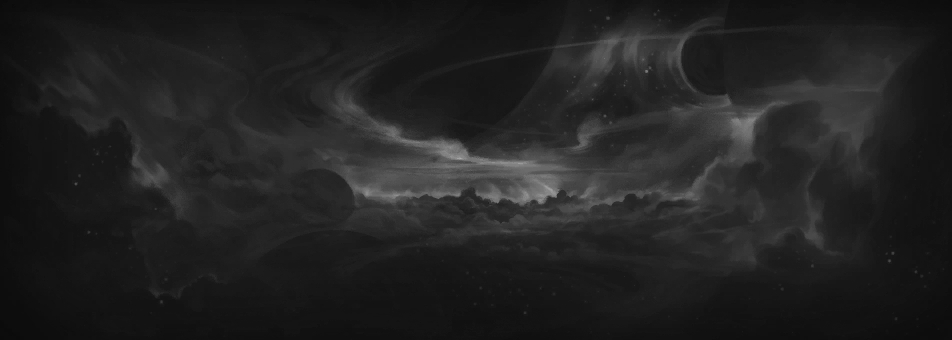
\includegraphics[width=1.0\linewidth]{pics/spth_dead_shroud_room.jpg}}
	
	\label{fig_touhou_dead_shroud}
\end{figure}


\newpage
\noindent {\zihao{5}\bf{附录·原案·契约}}

\adjustbox{trim=0pt {0.5\height} 0pt 0pt, clip}{妖怪居于大地，若灵力充盈，则地动山摇；衰微，则百物凋敝。}

\adjustbox{trim=0pt {0.5\height} 0pt 0pt, clip}{妖怪相斗，其势烈如焚火，恐致使天地崩坏。}

\adjustbox{trim=0pt {0.5\height} 0pt 0pt, clip}{然若毫无争斗，灵力必枯竭如旱泉。}

\adjustbox{trim=0pt {0.5\height} 0pt 0pt, clip}{我不会背弃，你们唯有遵从决斗之轨范，一切方闪耀永远。}

\adjustbox{trim=0pt 0pt 0pt {0.5\height}, clip}{八云紫即对众人言——}

\adjustbox{trim=0pt 0pt 0pt {0.5\height}, clip}{其一，妖怪当能轻易兴起异变，如风起于青萍，不滞于形}

\adjustbox{trim=0pt 0pt 0pt {0.5\height}, clip}{其一，人类当能轻易平复异变，如日光消晨露，不劳其力}

\adjustbox{trim=0pt 0pt 0pt {0.5\height}, clip}{其一，断然弃绝纯粹以力为尊之道，因其未必使众人和睦}

\adjustbox{trim=0pt 0pt 0pt {0.5\height}, clip}{其一，凡美丽之事，并思念之情，其权能超乎万有，无物可与之抗衡。}

\adjustbox{trim=0pt {0.5\height} 0pt 0pt, clip}{那境界妖怪一再叮嘱——}

\adjustbox{trim=0pt {0.5\height} 0pt 0pt, clip}{尔等当称决斗之荣美为名，又当赋予其义，使战非徒然。}

\adjustbox{trim=0pt {0.5\height} 0pt 0pt, clip}{决斗之前，必先宣告回合之数，以定为约；不可穷追猛打，直至气竭力尽。}

\adjustbox{trim=0pt {0.5\height} 0pt 0pt, clip}{凡无意义之攻，尔等当禁绝；惟有所指、有所托，力乃得坚。}

\adjustbox{trim=0pt {0.5\height} 0pt 0pt, clip}{若在命名之战中败北，纵余力尚存，亦当俯首认输；胜者不得戕害他者之性命。}

\adjustbox{trim=0pt {0.5\height} 0pt 0pt, clip}{决斗之名，当书于纸，如立契约之状，使此规坚不可破；其纸名曰“符卡”}

\adjustbox{trim=0pt {0\height} 0pt 0pt, clip}{至于决斗之细则，并施行之仪，尔等当往寻巫女，与她面议，她必指教你们当行的路。}

\adjustbox{trim=0pt 0pt 0pt {0\height}, clip}{此法亦不是终点，仅仅是起点，永为幻想乡之例，世代遵行，愿不再有苦难，不再有黑夜}

% \begin{multicols}{1}
\noindent {\zihao{5}\bf{附录·遗落于竹林之中的便签}}

% \adjustbox{trim=0pt {0.5\height} 0pt 0pt, clip}{夜晚的竹林是这么容易迷路的吗？}

\adjustbox{trim=0pt 0pt 0pt {0.5\height}, clip}{夜晚的竹林是这么容易迷路的吗？}

\adjustbox{trim=0pt 0pt 0pt {0.5\height}, clip}{手机没信号，GPS又没反应，}

\adjustbox{trim=0pt 0pt 0pt {0.5\height}, clip}{顺便找到了一些天然竹笋？}

\adjustbox{trim=0pt 0pt 0pt {0.5\height}, clip}{今天就在这附近休息吧……啊，现在是梦中吧？}

\adjustbox{trim=0pt 0pt 0pt {0.5\height}, clip}{那就再走走看吧。}

\adjustbox{trim=0pt 0pt 0pt {0.5\height}, clip}{说来今晚满天星星呢。}

\adjustbox{trim=0pt 0pt 0pt {0.5\height}, clip}{未开发的土地，清新的空气，就像很久以前的世界啊。}

\adjustbox{trim=0pt 0pt 0pt {0.5\height}, clip}{时间轮回了吗？霍金的时间逆转运行是真的吗？}

\adjustbox{trim=0pt 0pt 0pt {0.5\height}, clip}{如果这里没有妖怪就更好了。}

\adjustbox{trim=0pt 0pt 0pt {0.5\height}, clip}{对了，说不定梦境世界就是魂的构成物质的记忆呢。}

\adjustbox{trim=0pt 0pt 0pt {0.5\height}, clip}{而妖怪则是作为恐怖记忆的象征。}

\adjustbox{trim=0pt 0pt 0pt {0.5\height}, clip}{嗯，这是一种新见解呢。}

\adjustbox{trim=0pt 0pt 0pt {0.5\height}, clip}{醒后一定要和莲子说说。}

\adjustbox{trim=0pt 0pt 0pt {0.5\height}, clip}{那么，差不多该继续彷徨了。}

% \end{multicols}




%%%%%%%%%%%%%%%%%%%%%%%%%%%%%%%%%%%
%%%%%%%%%%%%%%%%%%%%%%%%%%%%%%%%%%%5

%\newpage

%\begin{multicols}{1}
%\begin{biography}[yourphotofilename.jpg]
%\noindent
%\textbf{First A. Author}\ \ 第1作者提供照片电子图片，尺寸为1寸。英文作者介绍内容包括：出生年,学位(或目前学历),职称,主要研究领域(\textbf{与中文作者介绍中的研究方向一致}).*
%*字体为小5号Times New Roman*
%\end{biography}

%\begin{biography}[yourphotofilename.jpg]
%\noindent
%\textbf{Second B. Author} *英文作者介绍内容包括：出生年,学位(或目前学历),职称,主要研究领域(\textbf{与中文作者介绍中的研究方向一致})。*
%*字体为小5号Times New Roman*
%\end{biography}
%\end{multicols}


% \begin{multicols}{1}
% \zihao{5}
% \noindent \textbf{Background}

% \zihao{5-}{
% \setlength\parindent{2em}
% *论文背景介绍为\textbf{英文}，字体为小5号Times New Roman体*

% 论文后面为400单词左右的英文背景介绍。介绍的内容包括：

% 本文研究的问题属于哪一个领域的什么问题。该类问题目前国际上解决到什么程度。

% 本文将问题解决到什么程度。

% 课题所属的项目。

% 项目的意义。

% 本研究群体以往在这个方向上的研究成果。

% 本文的成果是解决大课题中的哪一部分，如果涉及863$\backslash
% $973以及其项目、基金、研究计划，注意这些项目的英文名称应书写正确。}

% \end{multicols}

\end{document}


